% !TEX program = xelatex
% ============================================================================
% 基于随机预算训练的4D高斯泼溅可变预算渲染方法
% 目标期刊：The Visual Computer (Springer, sn-jnl format)
% 中文润色稿
% 编译建议：XeLaTeX -> BibTeX -> XeLaTeX -> XeLaTeX
% ============================================================================
\PassOptionsToPackage{unicode,breaklinks=true}{hyperref}
\documentclass[sn-mathphys]{sn-jnl}
\usepackage[UTF8]{ctex}
\usepackage{graphicx}
\usepackage{booktabs}
\usepackage{multirow}
\usepackage{array}
\usepackage{float}
\usepackage{placeins}
\usepackage{xurl}

% 避免 breakurl 在 XeLaTeX/dvipdfmx 流程下把 PostScript 片段打印到首页。
\makeatletter
\let\headerps@out\@empty
\makeatother

% 减少浮动体与正文之间的过大留白，并避免模板强制拉伸页面。
\raggedbottom
\setlength{\textfloatsep}{8pt plus 2pt minus 2pt}
\setlength{\floatsep}{8pt plus 2pt minus 2pt}
\setlength{\intextsep}{8pt plus 2pt minus 2pt}
\setlength{\abovecaptionskip}{4pt}
\setlength{\belowcaptionskip}{2pt}
\renewcommand{\arraystretch}{1.08}

\graphicspath{{figures/}}

% ============================================================================
\jyear{2026}
\title{基于随机预算训练的4D高斯泼溅可变预算渲染方法}

\author*[1,2]{\fnm{Guangzi} \sur{Zhang}}%
\author[2]{\fnm{Yulong} \sur{Pan}}%
\author[2]{\fnm{Xingquan} \sur{Cai}}%

\affil*[1]{\orgdiv{Beijing Key Laboratory of Cross-Modal Intelligent Immersive Computing}, \orgname{North China University of Technology}, \orgaddress{\city{Beijing}, \postcode{100144}, \country{China}}}
\affil[2]{\orgdiv{School of Artificial Intelligence and Computer Science}, \orgname{North China University of Technology}, \orgaddress{\city{Beijing}, \postcode{100144}, \country{China}}}

\abstract{
4D高斯泼溅（4DGS）是近年来动态场景重建与实时新视角合成领域的一项重要进展。然而，现有4DGS模型在训练完成后，基元数量通常已经固定，难以在算力差异较大的部署设备之间灵活切换。如果直接裁剪训练后的模型，虽然实现上较为简单，却容易破坏基元之间在训练中形成的协同关系，导致低预算渲染质量明显下降；若为每个目标预算分别训练模型，则会带来额外的训练、存储和维护成本。

本文关注一个简单但实际的问题：能否通过一次训练得到一个可按预算直接截取的4DGS模型，使其在不同基元数量下都保持可用的渲染质量？受Matryoshka表征学习及其在静态3D高斯泼溅中的应用启发，我们提出一种面向动态4DGS的随机预算训练策略。在训练过程中，模型随机采样不同的基元预算，并在部分训练迭代中以前缀基元作为主要监督对象进行预算约束优化，使模型在优化阶段主动适应不同稀疏程度的基元子集。

不过，将Matryoshka式思想从静态3DGS迁移到动态4DGS，并非直接替换即可完成。由于HexPlane变形场会随时间改写高斯基元的位置、尺度和不透明度，规范空间中的静态属性已难以准确反映基元在当前时刻的实际贡献。为此，我们设计了变形感知的重要度评分函数，以变形后的不透明度和屏幕空间覆盖面积代理共同衡量基元贡献，从而在预算截取时优先保留对动态渲染更关键的基元。

此外，我们还重新考察了预算分支中的损失设计和排序策略。实验观察表明，在动态场景中，仅对前缀基元施加渲染监督有助于减轻前缀监督与完整集监督在变形场优化中的潜在冲突；同时，多个测试场景中的基元重要度排序表现出较强的时间稳定性，使推理阶段可以采用一次性静态排序，而无需逐帧重新计算完整基元集合的重要度。

我们在多个合成与真实动态场景上验证了该方法。结果表明，相比训练后裁剪，本文方法在低预算条件下能够更稳定地保持渲染质量，并在降低基元数量时带来明显的渲染速度提升；在完整预算下，模型仍能维持与标准4DGS相近的视觉质量。该方法不引入额外可学习参数，训练开销较小，为4DGS模型在异构计算平台上的可变预算部署提供了一种轻量而实用的训练机制。
}

\keywords{4D高斯泼溅，随机预算训练，动态场景渲染，基元重要度评分，可变预算推理，层次细节}

% ============================================================================
\begin{document}

\maketitle

% ============================================================================
\section{引言}
\label{sec:intro}

从多视角图像或视频中重建动态三维场景，并实时合成高质量的新视角画面，是计算机视觉与计算机图形学中的一个核心问题。神经辐射场（NeRF）\cite{mildenhall2020nerf} 以隐式坐标网络建模场景几何与外观，在新视角合成任务上取得了显著进展，但其依赖密集光线采样和网络查询，往往难以满足实时渲染的需求。3D高斯泼溅（3DGS）\cite{kerbl20233dgaussians} 将场景表示转向显式的各向异性高斯基元，并通过GPU友好的可微光栅化实现高质量实时渲染，显著推动了神经渲染方法在实际应用中的可用性。

在此基础上，4D高斯泼溅方法\cite{wu20244dgaussians, yang2024deformable3dgs, yang2024realtime4dgs, duan20244drotor} 进一步将规范空间中的高斯表示与时间变形场结合，使基元能够随时间发生位移、旋转、缩放和不透明度变化，从而适应动态场景中的非刚性运动与时变外观。其中，基于HexPlane的4DGS框架通过紧凑的时空特征分解和显式高斯光栅化，在动态场景重建与实时新视角合成之间取得了较好的平衡。

然而，现有4DGS流程仍然存在一个容易被忽视的结构性局限：训练完成后，高斯基元数量通常已由自适应致密化与裁剪过程确定，模型容量随之固定。对于单一硬件环境，这种设定通常不会造成明显问题；但在实际部署中，同一动态场景可能需要运行在算力差异很大的设备上，例如桌面工作站、移动端芯片或VR/AR头显。此时，固定容量模型难以根据运行时资源灵活调整``质量---速度''之间的权衡。

一种直接的解决思路是在训练完成后裁剪低贡献基元\cite{fan2024lightgaussian, liu2025light4gs}，以降低渲染开销。然而，标准4DGS模型在训练过程中始终依赖完整基元集合进行优化，基元之间已经形成了隐式的互补关系。训练后直接移除部分基元，虽然实现简单，却可能破坏这种协同结构，尤其在低预算设置下造成明显的质量退化。另一种做法是为不同目标预算分别训练专用模型，但这会使训练时间、存储空间和模型维护成本随预算数量增加而增长，也不利于面向异构设备的灵活部署。

本文关注的正是这样一个简单但实际的问题：能否通过一次训练得到一个可按预算直接截取的4DGS模型，使其在不同基元数量下都保持可用的渲染质量？这一问题的关键不在于进一步压缩一个固定模型，而在于让模型在训练阶段就学会适应不同稀疏程度的基元子集，从而在推理阶段能够通过截取前缀基元实现可变预算渲染。

我们从Matryoshka表征学习\cite{kusupati2022matryoshka}及其在静态3D高斯泼溅中的应用---Matryoshka Gaussian Splatting（MGS）\cite{guo2026matryoshkagaussiansplatting}---中获得启发。MGS的核心思想是在训练过程中随机采样不同的表示预算，使模型在多种子集规模下共同优化；推理时，用户可以根据目标预算直接截取排序后的前缀基元。本文将这一思想扩展到动态4DGS中，提出一种面向4D高斯泼溅的随机预算训练策略。在部分训练迭代中，模型随机采样一个基元预算比例，根据重要度排序选择前缀基元进行预算约束监督，同时保留完整集渲染以维护致密化统计；其余迭代则保持完整基元集合的常规优化。通过这种方式，单一模型可以在训练过程中持续接触不同预算条件下的渲染任务，从而减轻推理时减少基元数量所造成的质量下降。

不过，将Matryoshka式训练思想从静态3DGS迁移到动态4DGS，并非简单替换底层表示即可完成。在静态3DGS中，高斯基元的几何和不透明度等属性在优化后相对固定，因此规范空间中的不透明度可以作为基元重要度的一个合理近似。但在基于HexPlane变形场的4DGS中，基元属性会随时间被动态改写：一个在规范空间中不透明度较高的基元，在特定时刻可能对最终图像贡献有限；反过来，一个不透明度中等但覆盖范围较大的基元，也可能在局部区域产生重要影响。因此，直接沿用静态MGS中的排序依据，难以准确反映动态场景中基元的逐时刻贡献。在初步实验中，我们观察到直接沿用不透明度排序的朴素MGS-4D在低预算条件下会出现明显退化；而引入变形感知评分后，bouncingballs场景在10\%预算下的PSNR由24.7 dB提升至32.1 dB。这一差异说明，动态4DGS中的基元重要度不能简单由规范空间中的静态属性决定，而需要结合变形后的逐时刻属性重新估计。

为此，本文设计了一种变形感知的重要度评分函数。该评分不再依赖规范空间中的静态属性，而是利用HexPlane变形后的不透明度和屏幕空间覆盖面积代理共同估计基元贡献。前者反映基元在当前时刻的可见性，后者近似其在图像空间中的影响范围。通过将二者结合，模型能够在预算截取时优先保留对动态渲染更关键的基元，从而提升低预算条件下的渲染稳定性。

除了重要度评分外，本文还重新考察了随机预算训练在动态场景中的损失设计与排序策略。与静态MGS中同时优化前缀渲染损失和完整集损失的做法不同，我们在动态4DGS中观察到，仅对前缀基元施加渲染监督有助于获得更稳定的低预算表现。这一现象提示，前缀监督与完整集监督在变形场优化中可能存在潜在的梯度目标差异。与此同时，我们发现多个测试场景中的基元重要度排序具有较强的时间稳定性，使推理阶段可以采用一次性静态排序，而无需逐帧重新计算完整基元集合的重要度。

我们在D-NeRF \cite{pumarola2021dnerf} 的多个合成动态场景和NeRF-DS \cite{cai2022nerfds} 的真实动态场景上对方法进行了评估。实验结果表明，相比训练后裁剪，本文方法在低预算条件下能够更稳定地保持渲染质量，并在降低基元数量时带来明显的渲染速度提升；在完整预算下，模型仍能维持与标准4DGS相近的视觉质量。由于该方法不引入额外可学习参数，也不改变原有的HexPlane变形场和高斯光栅化器，因此可以作为一种轻量的训练机制集成到现有4DGS框架中。

概括而言，本文的贡献包括以下四个方面：

\begin{itemize}
    \item 我们将随机预算训练从静态3D高斯泼溅扩展到基于HexPlane变形场的动态4DGS框架，使单一模型能够在推理阶段按照不同基元预算进行前缀截取，从而支持可变预算的新视角合成。
    \item 我们提出一种变形感知的重要度评分函数，利用变形后的不透明度与屏幕空间覆盖面积代理共同估计高斯基元在当前时刻的渲染贡献，避免直接依赖规范空间静态属性所带来的排序偏差。
    \item 我们重新考察了随机预算训练在动态4DGS中的损失设计，并采用纯前缀损失对预算约束下的基元子集进行直接监督。实验观察表明，这一设计有助于减轻前缀监督与完整集监督在变形场优化中的潜在冲突，使模型在低预算条件下获得更稳定的渲染表现。
    \item 我们分析了基元重要度排序在动态序列中的时间稳定性，并验证了一次性静态排序在所测试场景中的可行性。该观察使推理阶段无需逐帧重新计算完整基元集合的重要度，从而简化了可变预算渲染流程。
\end{itemize}

% ============================================================================
\section{相关工作}
\label{sec:related}

\subsection{动态场景渲染与4D高斯泼溅}

神经辐射场（NeRF）\cite{mildenhall2020nerf} 推动了新视角合成研究的发展。它使用坐标MLP表示场景的密度和颜色，可以在静态场景中生成高质量图像。但NeRF依赖沿光线的密集采样和网络查询，渲染效率较低。这个问题在动态场景中更加明显，因为模型还需要额外描述时间变化。

为处理动态内容，后续方法在NeRF框架中引入了时间建模。D-NeRF通过规范空间和变形场表示非刚性运动。HyperNeRF进一步处理拓扑变化。TiNeuVox使用体素特征提升训练和渲染效率。DynIBaR则结合图像特征和时序信息进行动态视图合成。这些方法增强了动态场景表达能力，但大多仍受限于隐式表示的采样成本。

3D高斯泼溅（3DGS）\cite{kerbl20233dgaussians} 将场景表示从隐式辐射场转向显式高斯基元。每个基元具有位置、尺度、旋转、不透明度和颜色等属性。渲染时，高斯基元被投影到图像空间，并通过可微光栅化完成alpha混合。由于这一过程更适合GPU并行计算，3DGS能够在保持较高图像质量的同时实现实时渲染。

动态高斯方法在3DGS基础上进一步引入时间维度。4DGaussians \cite{wu20244dgaussians} 在规范空间中维护一组高斯基元，并使用HexPlane变形场预测不同时刻的基元属性变化。类似工作还从变形建模~\cite{yang2024deformable3dgs,duan20244drotor}、实时渲染~\cite{yang2024realtime4dgs}、密度控制~\cite{cao2026spatiogs}和标签引导重建~\cite{wang2026label4dgs}等角度改进动态高斯表示。这些方法说明，显式高斯基元可以有效支持动态场景的新视角合成。

本文以基于HexPlane变形场的4DGS框架为基础，关注训练和推理阶段的基元选择机制，研究如何通过随机预算训练使同一个动态高斯模型适应不同的基元预算，并在质量与效率之间实现灵活权衡。

\subsection{高效高斯泼溅与模型压缩}

高斯基元数量与渲染速度、存储开销和显存占用密切相关。因此，压缩和加速一直是3DGS研究中的重要方向。

在静态场景中，LightGaussian \cite{fan2024lightgaussian} 通过重要度评估裁剪冗余高斯，并结合量化降低模型大小。Compact3D \cite{lee2024compact3d} 学习掩码和量化表示，以获得更紧凑的高斯模型。EAGLES \cite{girish2024eagles} 关注高效编码，使高斯表示更便于存储和传输。RadSplat \cite{niemeyer2024radsplat} 从alpha混合贡献出发组织高斯基元，以提升渲染效率。

动态4DGS中也出现了压缩和加速方法。Light4GS \cite{liu2025light4gs} 面向动态高斯模型进行轻量化。MEGA \cite{zhang2025mega} 关注内存效率和紧凑表示。4DGC \cite{hu20254dgc} 从率失真优化角度压缩4D高斯。PD-4DGS \cite{li2025pd4dgs} 则面向渐进传输和不同带宽条件组织动态高斯数据。DHO-3DGS \cite{zhang2026dho3dgs} 通过动态混合优化和极化损失剪枝实现紧凑3DGS。这些方法降低了4DGS的资源需求，也推动了动态高斯表示的实际应用。

上述方法大多以固定压缩率或固定资源配置为目标。也就是说，优化完成后，模型通常对应一个确定的容量。若目标设备或运行预算发生变化，往往需要重新选择压缩率，甚至重新优化模型。本文研究的是另一类问题：不是把模型压缩到某一个固定大小，而是让单一模型能够在推理阶段支持多个基元预算。

这一目标与后训练压缩方法是互补的。可变预算训练决定的是模型如何在不同前缀子集下保持可用质量；量化、编码和渐进传输则可以进一步降低每个预算点下的存储和带宽成本。因此，本文方法可以视为高效4DGS中的一种训练策略，而不是替代已有压缩技术的完整压缩框架。

\subsection{Matryoshka表示与可变预算推理}

Matryoshka表征学习\cite{kusupati2022matryoshka} 的核心思想是让同一个表示在不同维度或不同容量下都保持可用。模型在训练时同时接触多个表示尺度。推理时，可以根据计算预算截取表示的一部分，而不必重新训练模型。

这一思想已经被引入静态3D高斯泼溅。Matryoshka Gaussian Splatting（MGS）\cite{guo2026matryoshkagaussiansplatting} 在训练过程中随机采样基元预算，并按照重要度选择前缀高斯进行渲染监督。训练完成后，用户可以直接截取排序后的前缀基元，以获得不同质量和速度的渲染结果。MGS证明了可变预算思想在静态3DGS中的可行性。

本文与MGS关系最为直接。我们同样希望通过一次训练得到一个支持多预算推理的高斯模型。但本文处理的是动态4DGS，而不是静态3DGS。这一区别带来了新的问题。在静态场景中，高斯属性在训练后基本固定，基元排序可以依赖规范空间中的静态属性。而在4DGS中，HexPlane变形场会随时间修改基元的位置、尺度和不透明度。静态排序准则因此可能不再可靠。

此外，随机预算训练与动态变形场之间也存在更复杂的优化关系。前缀子集需要在低预算下独立完成渲染，而完整基元集合又需要维持高容量下的质量。两类监督信号可能对变形场产生不同的优化压力。因此，本文在借鉴MGS训练思想的同时，重新设计了动态场景中的重要度评分，并重新考察了预算分支中的损失形式。

\subsection{预算约束下的基元重要度估计}

可变预算渲染需要对高斯基元进行排序。排序的目标是让更重要的基元出现在前缀中。这样，当预算降低时，模型仍能保留对图像贡献较大的部分。

已有高斯压缩方法采用了不同的重要度估计方式。部分方法使用学习得到的掩码选择基元。部分方法根据几何属性、透明度或渲染贡献设计启发式评分。也有方法直接分析alpha混合过程中的贡献，估计每个高斯对最终图像的影响。这些策略能够有效减少冗余，但通常服务于固定压缩目标。

本文中的重要度估计需要满足两个条件。第一，它要适合动态4DGS。基元的重要性不应只由规范空间属性决定，而应考虑变形后的逐时刻属性。第二，它要足够轻量。随机预算训练会反复执行排序和截取，如果评分过程过于复杂，会增加训练开销。

基于这一考虑，本文采用无参数的变形感知评分。该评分结合变形后的不透明度和屏幕空间覆盖面积代理。不透明度表示当前时刻的可见性，面积代理表示基元在图像中的影响范围。与纯不透明度排序相比，这一评分更适合动态高斯基元随时间改变尺度和贡献的情况。与学习式评分相比，它不引入额外网络，也不需要独立训练阶段。

% ============================================================================
\section{方法}
\label{sec:method}

本文方法建立在4DGaussians \cite{wu20244dgaussians} 之上，并在其动态高斯表示框架中引入随机预算训练机制，使同一个4DGS模型能够在推理阶段按照不同基元预算进行前缀截取。以下先简述基础4DGS表示与渲染流程，随后介绍随机预算训练、变形感知重要度评分、纯前缀损失与致密化统计，以及排序时间稳定性的观察。

\subsection{预备知识：4D高斯泼溅}
\label{sec:prelim}

4DGaussians在规范空间中维护一组三维高斯基元。第 $i$ 个高斯基元由位置 $\mu_i$、尺度 $s_i$、旋转 $q_i$、不透明度 $\alpha_i$ 和颜色特征 $c_i$ 等属性表示。其中，尺度和旋转共同决定高斯协方差，颜色通常由球谐系数建模，以支持视角相关外观。

为了表示动态场景，4DGaussians使用时间条件变形场预测不同时刻的基元属性变化。给定时间戳 $t$，HexPlane变形场 $D_{\phi}$ 将规范空间中的高斯属性和逐基元特征映射为属性偏移：

\begin{equation}
\{\Delta \mu_i, \Delta s_i, \Delta q_i, \Delta \alpha_i\}
=
D_{\phi}(\mu_i, s_i, q_i, \alpha_i, f_i, t),
\label{eq:deformation}
\end{equation}

其中 $f_i$ 表示额外的逐基元可学习特征。变形后的高斯属性可写为：

\begin{equation}
\tilde{\mu}_i(t)=\mu_i+\Delta \mu_i(t),
\end{equation}

\begin{equation}
\tilde{s}_i(t)=s_i+\Delta s_i(t),
\end{equation}

\begin{equation}
\tilde{q}_i(t)=q_i+\Delta q_i(t),
\end{equation}

\begin{equation}
\tilde{\alpha}_i(t)=\alpha_i+\Delta \alpha_i(t).
\end{equation}

随后，变形后的高斯基元被投影到图像空间，并按照深度顺序进行alpha混合。对于给定像素，其渲染颜色可以表示为：

\begin{equation}
C =
\sum_i c_i(d)\,\tilde{\alpha}_i
\prod_{j=1}^{i-1}(1-\tilde{\alpha}_j),
\label{eq:rendering}
\end{equation}

其中 $c_i(d)$ 表示与视角方向 $d$ 相关的颜色，$\tilde{\alpha}_i$ 表示变形后的有效不透明度。基础4DGS训练通常交替执行优化、致密化和裁剪，并最小化 $L_1$ 与D-SSIM组成的图像重建损失：

\begin{equation}
\mathcal{L}_{\mathrm{rec}}
=
(1-\lambda)\mathcal{L}_1
+
\lambda \mathcal{L}_{\mathrm{D\text{-}SSIM}},
\label{eq:loss}
\end{equation}

其中 $\lambda$ 为D-SSIM损失权重。

本文不修改HexPlane变形场、高斯参数化方式或可微光栅化器。我们的改动集中在训练阶段的预算约束监督和推理阶段的基元子集选择上。

\subsection{随机预算训练}
\label{sec:sbt}

标准4DGS在每次训练迭代中使用完整高斯集合进行渲染。训练完成后，模型中的基元数量由致密化和裁剪过程确定，推理时通常也使用全部基元。这样的流程无法直接支持不同计算预算下的灵活截取。

为此，本文引入随机预算训练。每次训练迭代首先从均匀分布中采样随机数 $u \sim U(0,1)$。若 $u < p_{\mathrm{mgs}}$，当前迭代进入预算约束分支；否则执行常规完整集训练。实验中设置：

\begin{equation}
p_{\mathrm{mgs}} = 0.5.
\end{equation}

在预算约束分支中，我们从区间 $[\rho_{\min}, \rho_{\max}]$ 内均匀采样预算比例：

\begin{equation}
\rho \sim U(\rho_{\min}, \rho_{\max}),
\end{equation}

并根据当前高斯基元总数 $N$ 计算保留数量：

\begin{equation}
K = \max(2, \lfloor \rho N \rfloor).
\end{equation}

实验中设置 $\rho_{\min}=0.1$，$\rho_{\max}=1.0$，使训练过程覆盖从低预算到完整预算的不同基元规模。最小下限用于避免极低预算下出现空子集或退化子集。

随后，模型根据当前时刻的基元重要度对所有高斯基元进行排序，并选择排名靠前的 $K$ 个基元作为前缀子集。该前缀子集用于预算约束下的图像重建监督，使模型在训练阶段持续接触不同稀疏程度的渲染任务。

\begin{figure}[!htbp]
\centering
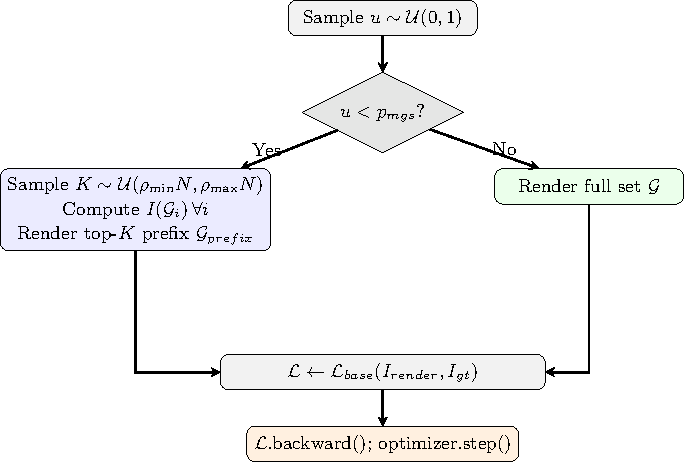
\includegraphics[width=0.85\textwidth]{fig_training_flow.pdf}
\caption{随机预算训练流程。每次训练迭代首先采样随机变量 $u$，并根据 $u < p_{\mathrm{mgs}}$ 判断是否进入预算约束分支。若进入预算分支，则采样基元预算，计算所有高斯基元的重要度，并选择排序后的前缀基元进行预算约束渲染。同时，完整基元集合仍被渲染，用于收集致密化统计信息。}
\label{fig:training_flow}
\end{figure}

需要注意的是，预算约束分支并不等价于完全丢弃未选中的基元。实际训练中，预算分支包含两类渲染：一类是只使用前 $K$ 个基元的前缀渲染，用于计算预算约束下的图像重建损失；另一类是使用完整基元集合的完整集渲染，用于保留原始4DGS训练过程中的致密化统计信息。也就是说，随机预算训练改变的是图像监督的主要对象，而不是完全移除完整集渲染在训练流程中的作用。

在本文采用的纯前缀损失配置下，完整集渲染主要用于提供投影半径和可见性过滤等致密化统计信息，而图像重建损失来自前缀渲染结果。这样可以在强化前缀子集低预算表达能力的同时，尽量保持原始4DGS致密化流程的稳定性。

推理阶段则更加直接。给定目标预算比例 $r \in (0,1]$，模型根据预先计算的重要度排序截取前 $\lfloor rN \rfloor$ 个高斯基元，并仅使用该前缀子集进行渲染。虽然该机制理论上支持任意连续预算比例，实验中我们主要在 $r \in \{0.1,0.25,0.5,0.75,1.0\}$ 五个预算点上进行定量评估。

\subsection{变形感知重要度评分}
\label{sec:importance}

随机预算训练的关键在于基元排序。排序决定了在低预算下哪些高斯基元会被保留，也直接影响前缀子集的渲染质量。

在静态3DGS中，高斯基元的属性在训练后相对固定。因此，规范空间中的不透明度可以作为基元贡献的一个简单近似。Matryoshka Gaussian Splatting（MGS）正是利用类似的静态重要度准则对基元进行排序。

然而，在动态4DGS中，这一假设不再充分。HexPlane变形场会根据时间戳改写高斯基元的位置、尺度、旋转和不透明度。一个在规范空间中不透明度较高的基元，在某个时刻可能并不显著；反过来，一个不透明度中等但空间覆盖范围较大的基元，也可能在局部区域中产生重要影响。因此，直接沿用静态MGS中的不透明度排序，难以准确反映动态场景中基元的逐时刻贡献。

为此，本文采用变形感知的重要度评分。给定时间戳 $t$，第 $i$ 个高斯基元的重要度定义为：

\begin{equation}
I(G_i,t)
=
\tilde{\alpha}_i(t)
\cdot
\tilde{s}_{i,x}(t)
\cdot
\tilde{s}_{i,y}(t),
\label{eq:importance}
\end{equation}

其中 $\tilde{\alpha}_i(t)$ 表示HexPlane变形后的不透明度，$\tilde{s}_{i,x}(t)$ 和 $\tilde{s}_{i,y}(t)$ 表示变形后尺度向量的前两个分量。这里使用 $\tilde{s}_{i,x}(t)\cdot \tilde{s}_{i,y}(t)$ 作为屏幕空间覆盖面积的轻量代理，而不是显式计算完整投影协方差。

该评分由两个部分组成。不透明度项反映基元在当前时刻的可见性，面积代理反映其在图像空间中的影响范围。二者结合后，可以更好地估计动态高斯基元在当前帧中的渲染贡献。

这一设计具有三个特点。第一，它直接使用变形后的属性，因此能够感知动态场景中的时变变化。第二，它不引入额外网络或可学习参数，计算过程可以直接附着在变形网络前向传播之后。第三，它足够轻量，适合在随机预算训练中反复执行排序和截取操作。

在后续消融实验中，我们将该评分与纯不透明度排序和随机排序进行比较，以验证空间覆盖面积代理在动态预算渲染中的作用。

\subsection{纯前缀损失与致密化统计}
\label{sec:loss}

MGS在预算分支中同时使用前缀渲染损失和完整集渲染损失，并通过权重系数 $f_w$ 对二者进行联合优化。我们在动态4DGS中重新考察这一设计，发现完整集损失并不一定有利于预算约束下的优化。

在本文的预算约束迭代中，训练过程包含两次渲染。第一次是前缀渲染，仅使用按重要度排序后的前 $K$ 个高斯基元；第二次是完整集渲染，仍然使用全部高斯基元。前缀渲染结果用于计算预算约束下的图像重建损失。完整集渲染则用于收集自适应致密化过程中所需的统计信息，例如投影半径和可见性过滤结果。

这一设计是为了保持原始4DGS致密化流程的稳定性。如果在预算分支中只执行前缀渲染，那么未被选中的基元无法在该迭代中提供完整的可见性和尺度统计，可能影响后续的致密化与裁剪。因此，完整集渲染在预算约束分支中仍然保留，但它并不参与本文的图像重建损失。

本文采用纯前缀损失配置。也就是说，在预算约束分支中，图像重建损失仅由前缀渲染结果计算：

\begin{equation}
\mathcal{L}_{\mathrm{budget}}
=
\mathcal{L}_{\mathrm{rec}}(R(G_{1:K}), I_{\mathrm{gt}}),
\label{eq:budget_loss}
\end{equation}

其中 $G_{1:K}$ 表示排序后的前 $K$ 个高斯基元，$R(\cdot)$ 表示渲染函数，$I_{\mathrm{gt}}$ 表示真实图像。

若写成包含完整集损失的形式，则可以表示为：

\begin{equation}
\mathcal{L}
=
\mathcal{L}_{\mathrm{prefix}}
+
f_w \mathcal{L}_{\mathrm{full}}.
\end{equation}

本文主要采用：

\begin{equation}
f_w = 0.
\end{equation}

在该设置下，完整集渲染仍然执行，但其图像重建损失不参与优化。因此，未被前缀选中的基元不会从当前迭代的图像重建损失中接收梯度；但它们仍然可以通过完整集渲染为致密化统计提供信息。

这一设计与静态MGS中的联合损失有所不同。动态4DGS中的前缀子集需要在低预算条件下独立完成渲染，而完整基元集合则倾向于维持高容量下的整体质量。二者可能对变形场产生不同的优化压力。纯前缀损失使预算分支的监督更加集中，鼓励模型优先提升前缀基元在低预算下的表达能力。消融实验显示，在本文测试的场景中，纯前缀损失相比联合损失获得了更稳定的低预算表现。

\subsection{排序的时间稳定性}
\label{sec:static}

由于4DGS中的高斯属性会随时间变化，一个自然的问题是：基元重要度排序是否也需要逐帧重新计算。如果排序在不同时间戳之间显著变化，那么推理阶段就必须在每一帧对完整基元集合重新计算重要度，这会带来额外开销。

为分析这一问题，本文比较了两种排序策略。第一种是时间自适应排序。该策略在每个测试帧的时间戳上重新计算所有高斯基元的重要度，并据此选择前缀子集。第二种是静态排序。该策略仅在参考时间 $t=0$ 计算一次重要度排序，并在后续所有帧中复用该排序结果。

实验结果显示，在本文测试的三个代表性场景中，静态排序与时间自适应排序产生了完全一致的前缀选择。两种策略在25\%预算下的PSNR完全相同，Kendall $\tau$ 秩相关系数均为1.0000，top-25\%基元重叠率达到100\%。这一结果表明，在本文测试的场景和预算设置下，基元重要度排序并未随时间发生可观测变化。

基于这一观察，推理阶段可以采用一次性静态排序，而无需逐帧对完整基元集合重新计算重要度。需要注意的是，静态排序只省去了完整集合上的逐帧重要度评估；渲染时，变形网络仍然需要对被选中的前缀基元运行，以获得当前时刻的位置、尺度、旋转和不透明度等变形后属性。对于更长序列、剧烈非刚性运动或拓扑变化明显的场景，排序稳定性仍可能受到影响，后续工作可进一步评估其适用范围。

\subsection{训练与推理流程总结}
\label{sec:summary}

综合上述设计，本文的训练流程可以概括如下。

在常规完整集训练迭代中，模型使用全部高斯基元进行渲染，并按照基础4DGS流程计算图像重建损失、更新高斯属性和变形场参数，同时维护致密化统计。

在预算约束训练迭代中，模型首先根据当前时间戳计算所有高斯基元的变形后属性，并利用变形感知评分得到重要度排序。随后，模型采样预算比例并截取前 $K$ 个高斯基元作为前缀子集。前缀子集用于预算约束下的图像重建监督。与此同时，完整基元集合仍然执行一次渲染，用于收集投影半径和可见性过滤等致密化统计信息。最终，在纯前缀损失配置下，梯度主要来自前缀渲染损失，而完整集渲染主要服务于致密化流程。

推理阶段不再进行随机预算采样。给定目标预算比例 $r$，模型直接根据静态排序截取前 $\lfloor rN \rfloor$ 个高斯基元，并对这些基元运行变形网络和光栅化渲染。这样，同一个训练好的4DGS模型即可在不同基元预算下运行，从而在渲染质量和计算效率之间进行灵活切换。

本文方法的核心在于通过随机预算训练，使模型在训练阶段持续接触不同预算下的前缀基元子集，从而提升低预算条件下的渲染质量；通过变形感知重要度评分，对动态场景中的高斯基元进行排序；通过纯前缀损失与完整集致密化统计的分离，使预算约束优化与原有致密化流程协同进行；并利用排序的时间稳定性，在推理阶段直接复用静态排序结果，实现不同预算下的灵活渲染。

% ============================================================================
\section{实验}
\label{sec:experiments}

本章从渲染质量、预算适应性、关键设计和计算效率四个方面评估本文方法。实验围绕三个问题展开：第一，随机预算训练是否能够提升低预算条件下的渲染质量；第二，单一模型是否能够在多个预算点上保持稳定表现；第三，变形感知评分、纯前缀损失和静态排序等设计是否对动态4DGS的可变预算渲染起到实际作用。

\subsection{实验设置}
\label{sec:setup}

\textbf{数据集。}
我们在9个动态场景上进行评估，包括D-NeRF的7个合成场景和NeRF-DS的2个真实场景。D-NeRF场景包括 bouncingballs、standup、mutant、trex、jumpingjacks、hook 和 hellwarrior，分辨率为 $800 \times 800$。NeRF-DS场景包括 plate 和 press，用于评估方法在真实采集和复杂视角相关外观条件下的表现。

\textbf{对比方法。}
共涉及四类配置：

\begin{enumerate}
    \item \textbf{标准4DGaussians。} 不施加任何预算约束，按照原始4DGS流程训练，并在推理时使用完整基元集合。
    \item \textbf{训练后裁剪。} 在标准模型训练完成后，使用与本文相同的重要度评分选取前 $K$ 个基元，但模型本身未经历预算约束训练。
    \item \textbf{朴素MGS-4D。} 将MGS直接迁移到4DGS框架中，使用纯不透明度排序和联合损失。
    \item \textbf{逐预算训练。} 为每个目标预算独立训练专用模型，用于比较单一可变预算模型与专用预算模型之间的差异。
\end{enumerate}

\textbf{训练配置。}
所有模型均使用相同的4DGS基础框架和HexPlane变形骨干。空间平面分辨率设为 $64^3$，特征通道数为32，使用单层MLP解码器和4个多分辨率层级。训练总迭代数为30,000次，其中粗阶段3,000次、精阶段27,000次。优化器和学习率调度与4DGaussians保持一致。

本文方法的随机预算训练参数设置为 $p_{\mathrm{mgs}}=0.5$，$\rho_{\min}=0.1$，$\rho_{\max}=1.0$，并采用纯前缀损失配置 $f_w=0$。所有实验均在单张 NVIDIA RTX 4080 SUPER GPU 上完成。

\textbf{评价指标。}
渲染质量使用PSNR、SSIM和LPIPS进行评估，其中LPIPS采用AlexNet骨干。效率方面报告端到端渲染帧率、单次迭代时间、总训练时间和峰值GPU显存。预算条件实验在 $r \in \{0.1,0.25,0.5,0.75,1.0\}$ 五个预算比例上进行。

\textbf{重复性验证。}
为了检查训练和评估流程的稳定性，我们在 bouncingballs 场景上使用随机种子42、123和2024进行重复训练。五个预算点上的PSNR和SSIM方差均保持在很小范围内，说明当前实现具有较好的实验稳定性。

\subsection{主要结果}
\label{sec:main}

\subsubsection{低预算渲染质量}

表~\ref{tab:main_25}比较了本文方法与训练后裁剪在25\%预算下的表现。本文方法在全部9个场景上均取得PSNR提升，平均增益为+2.0 dB。单场景提升范围从 jumpingjacks 的+1.0 dB 到 bouncingballs 的+3.7 dB。standup、mutant、hook、hellwarrior、plate 和 press 等场景也保持了稳定增益。

\begin{table}[!htbp]
\caption{25\%预算下本文方法与训练后裁剪的定量比较。两种方法使用相同的重要度评分；$\Delta$PSNR表示随机预算训练带来的优势。}
\label{tab:main_25}
\centering
\small
\setlength{\tabcolsep}{3.2pt}
\begin{tabular}{lccc|ccc|c}
\toprule
场景 & \multicolumn{3}{c}{训练后裁剪 (25\%)} & \multicolumn{3}{c}{本文方法 (25\%)} & $\Delta$PSNR \\
& PSNR$\uparrow$ & SSIM$\uparrow$ & LPIPS$\downarrow$ & PSNR$\uparrow$ & SSIM$\uparrow$ & LPIPS$\downarrow$ & \\
\midrule
bouncingballs & 35.14 & 0.9906 & 0.0229 & \textbf{38.82} & \textbf{0.9933} & \textbf{0.0130} & +3.7 \\
standup       & 33.70 & 0.9787 & 0.0143 & \textbf{36.09} & \textbf{0.9869} & \textbf{0.0117} & +2.4 \\
mutant        & 31.90 & 0.9670 & 0.0198 & \textbf{35.10} & \textbf{0.9807} & \textbf{0.0179} & +3.2 \\
trex          & 31.33 & 0.9746 & 0.0253 & \textbf{32.45} & \textbf{0.9810} & \textbf{0.0206} & +1.1 \\
jumpingjacks  & 32.71 & 0.9776 & 0.0223 & \textbf{33.67} & \textbf{0.9814} & \textbf{0.0221} & +1.0 \\
hook          & 29.79 & 0.9602 & 0.0280 & \textbf{31.57} & \textbf{0.9705} & \textbf{0.0241} & +1.8 \\
hellwarrior   & 26.08 & 0.9582 & 0.0449 & \textbf{28.06} & \textbf{0.9701} & \textbf{0.0381} & +2.0 \\
\midrule
plate (真实)  & 15.82 & 0.616  & --     & \textbf{17.10} & \textbf{0.663}  & --       & +1.3 \\
press (真实)  & 20.33 & 0.740  & 0.157  & \textbf{22.34} & \textbf{0.779}  & \textbf{0.125} & +2.0 \\
\midrule
平均 (9场景)  & 28.53 & 0.904  & --     & \textbf{30.58} & \textbf{0.923}  & --       & +2.0 \\
\bottomrule
\end{tabular}
\end{table}

这一结果说明，随机预算训练使前缀基元在训练阶段获得了直接监督。当推理阶段只保留部分基元时，模型能够更好地利用排序靠前的高斯子集完成渲染。训练后裁剪虽然使用相同的重要度评分，但其优化过程主要围绕完整基元集合展开，因此在低预算截取后更容易出现质量下降。

\begin{figure}[!htbp]
\centering
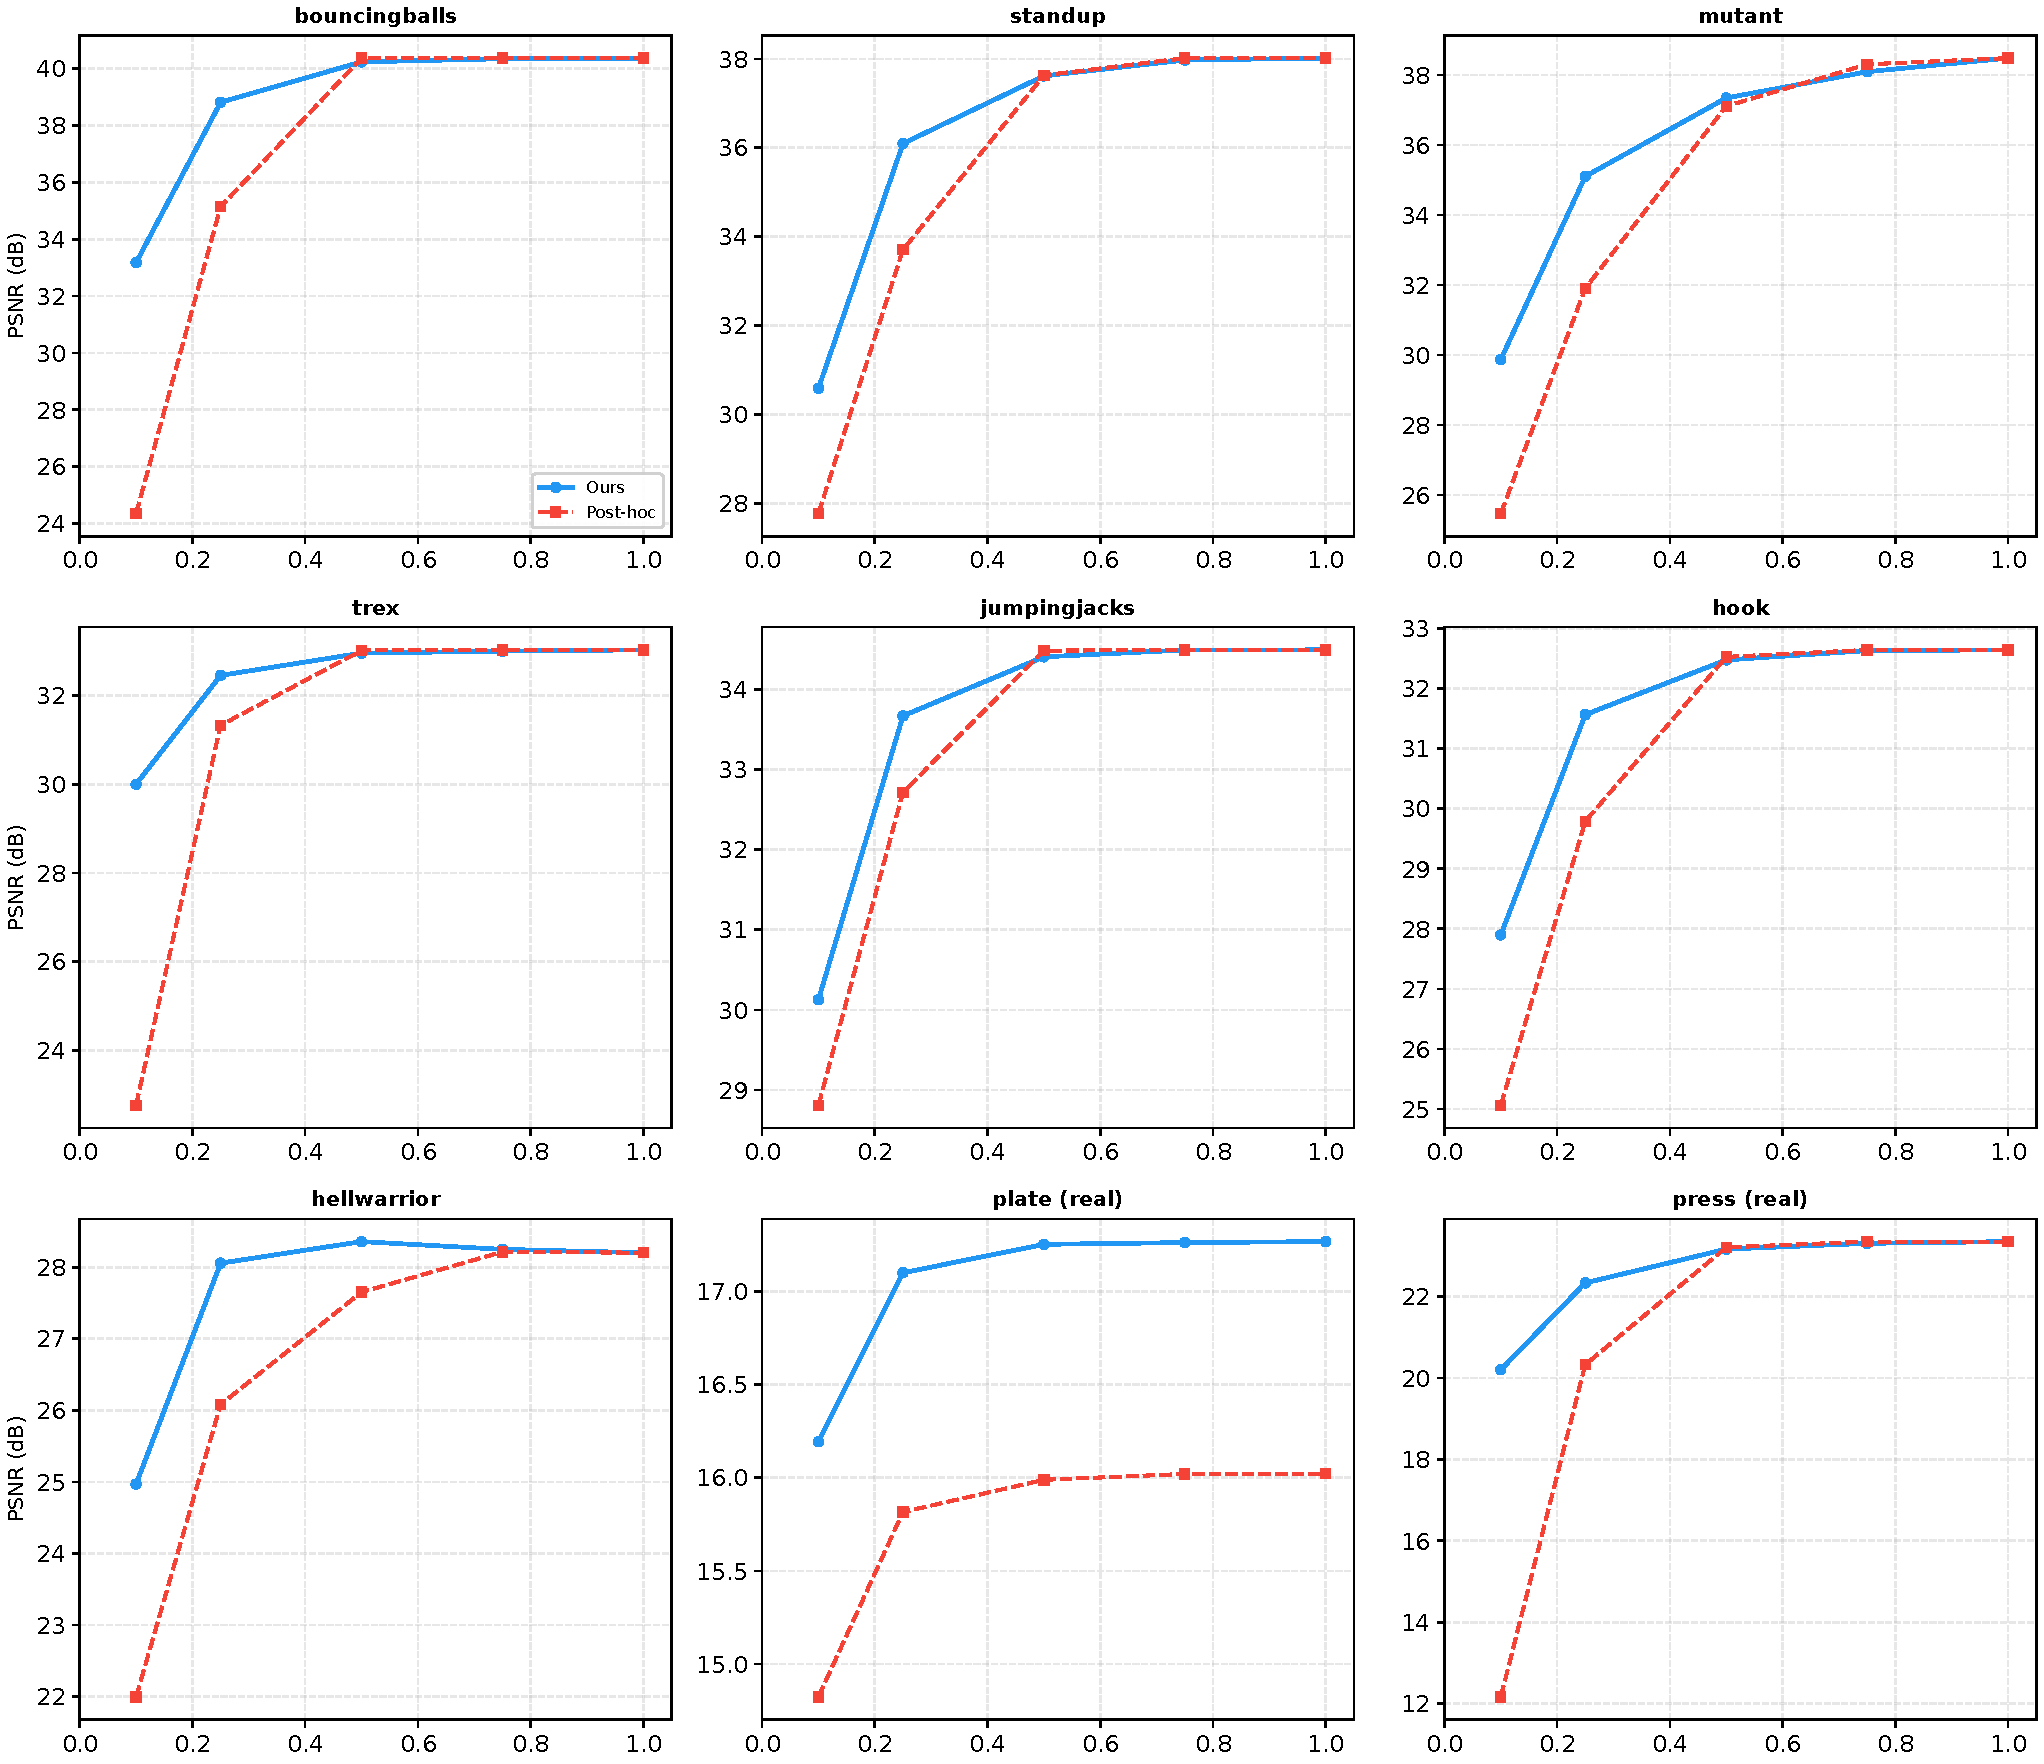
\includegraphics[width=0.86\textwidth]{fig2_all_budget_curves.pdf}
\caption{九个动态场景上的预算-质量曲线。横轴为保留的高斯基元预算比例，纵轴为PSNR。本文方法在多数合成和真实动态场景中均优于训练后裁剪，尤其在10\%至50\%预算区间内优势更明显。}
\label{fig:budget_curve}
\end{figure}

图~\ref{fig:budget_curve}展示了9个场景上的完整预算-质量曲线。可以看到，本文方法在低预算区域具有最明显优势。对于 bouncingballs、standup 和 mutant 等大幅动态场景，训练后裁剪在10\%和25\%预算下退化较明显，而本文方法保持了更高PSNR。对于 trex、jumpingjacks、hook 和 hellwarrior 等具有复杂运动的场景，本文方法同样在低预算区域取得稳定提升。两个真实场景 plate 和 press 的结果说明，随机预算训练也能改善真实采集条件下的低预算渲染质量。

随着预算比例提高，两种方法的曲线逐渐接近。这一趋势符合可变预算渲染的预期：低预算时，模型更依赖排序靠前的前缀基元，因此训练阶段的预算约束监督会带来更明显收益；高预算时，更多基元参与渲染，两种策略之间的差距自然缩小。

为更直观地观察低预算条件下的渲染差异，图~\ref{fig:visual_comparison}给出了两个代表性场景在25\%预算下的视觉比较。bouncingballs 为合成场景，物体运动较为规律，能够反映方法在典型动态合成数据上的表现；press 为真实镜面反射场景，包含复杂视角相关外观，能够反映方法在真实采集条件下的局限性。

\begin{figure}[!htbp]
\centering
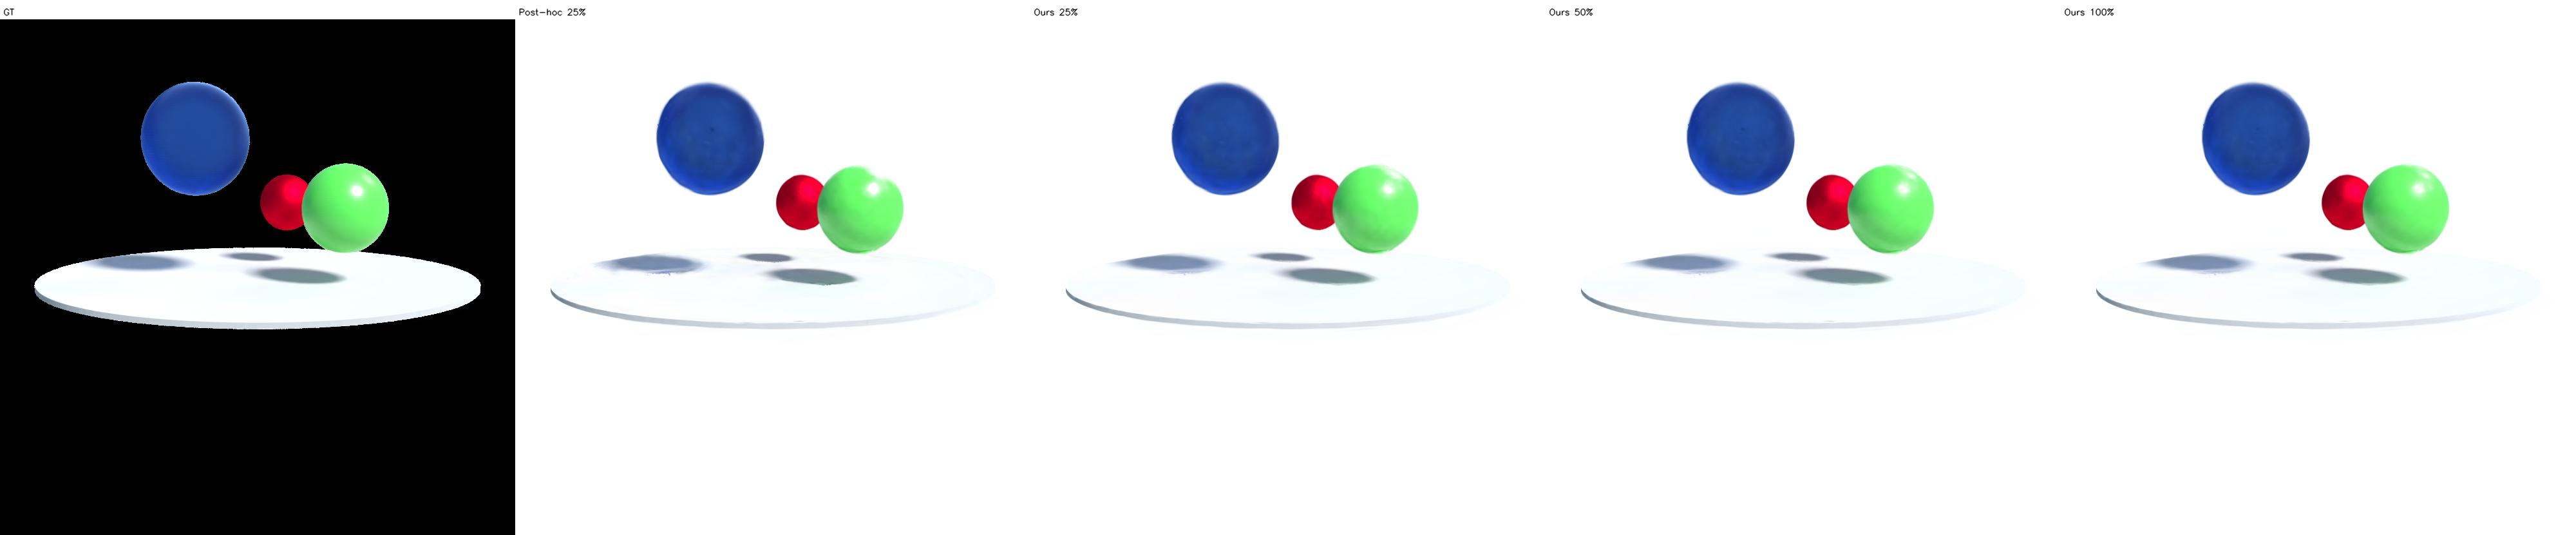
\includegraphics[width=0.95\textwidth]{fig3_vis_bouncingballs.png}
\vspace{4pt}
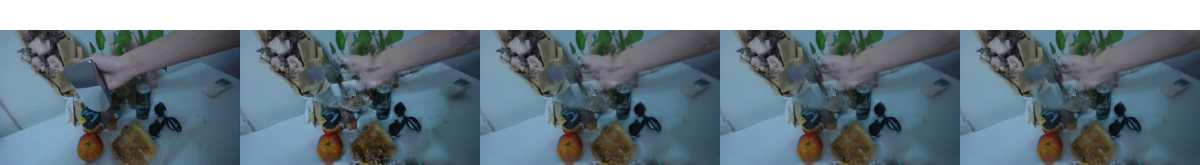
\includegraphics[width=0.95\textwidth]{fig3_vis_press.png}
\caption{25\%预算下本文方法与训练后裁剪的视觉比较。每列分别为 Ground Truth、本文方法（25\%预算）和训练后裁剪（25\%预算）。上方为 bouncingballs 合成场景（$\Delta$PSNR = +3.7 dB），下方为 press 真实镜面反射场景（$\Delta$PSNR = +2.0 dB）。}
\label{fig:visual_comparison}
\end{figure}

从 bouncingballs 的对比中可以观察到，本文方法在仅保留四分之一基元的情况下，仍能较好地恢复球体的形状、纹理和阴影细节，与 Ground Truth 的整体一致性较高；训练后裁剪虽然在球体主体区域保持了大体轮廓，但在边缘和阴影区域出现了更明显的模糊与畸变。这一差异印证了定量结果：随机预算训练使排序靠前的前缀基元在训练阶段持续接触低预算渲染，从而在推理截取后具备更强的独立表达能力。训练后裁剪中评分靠前的基元虽然在完整模型中发挥了作用，但由于从未在没有辅助基元配合的条件下独立承担渲染任务，截取后更容易出现局部退化。

press 场景的对比则呈现出不同的特点。该场景含有较强的镜面高光和视角相关反射，整体重建难度更高。在25\%预算下，本文方法的 PSNR 相较训练后裁剪提升了+2.0 dB，但从视觉上看，两种方法与 Ground Truth 之间均存在较明显的差距。本文方法在前景物体结构上更为清晰，排水口和金属表面的大致形态得以保留，但高光区域的细节恢复仍然不足；训练后裁剪则在物体边缘和背景区域出现了更多伪影，部分高光区域呈现块状或弥散状退化。这一现象与前文 press 场景中朴素 MGS-4D 反而优于本文方法的结果趋势一致，说明真实镜面反射场景中的基元重要度排序受到视角相关外观的显著影响——高光区域的关键基元往往被面积代理过度稀释，而部分外观关键基元在预算截取时被过早剔除。变形感知评分在当前形式下更偏向几何覆盖与可见性的结合，对外观敏感性的建模尚有进一步提升空间。

\subsubsection{完整预算性能}

在100\%预算下，本文方法使用全部高斯基元进行渲染。表~\ref{tab:main_full}报告了D-NeRF七个合成场景上的完整预算结果。与标准4DGS相比，本文方法的平均PSNR略有下降，但LPIPS从0.0204改善至0.0140，说明随机预算训练在完整预算下仍能保持良好的感知质量。

\begin{table}[!htbp]
\caption{100\%完整预算下标准4DGS与本文方法的定量比较。平均PSNR下降0.56 dB，但LPIPS从0.0204改善至0.0140。}
\label{tab:main_full}
\centering
\small
\setlength{\tabcolsep}{4pt}
\begin{tabular}{lccc|ccc}
\toprule
场景 & \multicolumn{3}{c}{标准4DGS (100\%)} & \multicolumn{3}{c}{本文方法 (100\%)} \\
& PSNR$\uparrow$ & SSIM$\uparrow$ & LPIPS$\downarrow$ & PSNR$\uparrow$ & SSIM$\uparrow$ & LPIPS$\downarrow$ \\
\midrule
bouncingballs & 40.72 & 0.9944 & 0.0141 & 40.37 & 0.9945 & 0.0092 \\
standup       & 38.62 & 0.9906 & 0.0124 & 38.02 & 0.9917 & 0.0061 \\
mutant        & 38.02 & 0.9890 & 0.0149 & 38.48 & 0.9926 & 0.0046 \\
trex          & 34.52 & 0.9857 & 0.0201 & 33.03 & 0.9837 & 0.0168 \\
jumpingjacks  & 35.54 & 0.9854 & 0.0197 & 34.49 & 0.9851 & 0.0171 \\
hook          & 33.04 & 0.9767 & 0.0253 & 32.65 & 0.9776 & 0.0164 \\
hellwarrior   & 28.68 & 0.9730 & 0.0362 & 28.20 & 0.9727 & 0.0277 \\
\midrule
平均 (7场景)  & 35.59 & 0.9850 & 0.0204 & 35.03 & 0.9854 & 0.0140 \\
\bottomrule
\end{tabular}
\end{table}

这一现象表明，预算约束训练在增强低预算前缀表达能力的同时，也保留了完整模型的整体渲染质量。模型在训练阶段反复使用不同规模的前缀基元进行渲染，使排序靠前的基元承担更稳定的表达责任。这种训练方式在低预算下带来直接收益，同时在完整预算下维持了与标准4DGS相近的视觉质量。

\subsubsection{多预算稳定性}

除单一预算点外，本文还比较了不同预算比例下的整体表现。图~\ref{fig:budget_curve}显示，本文方法在10\%、25\%、50\%、75\%和100\%预算之间形成了较平滑的质量变化曲线。这说明模型能够根据运行时预算逐步调整渲染质量，而不是只在某一个固定预算点上有效。

这一性质对异构设备部署具有实际意义。同一动态场景模型可以在高性能GPU上使用较高预算，以获得更高渲染质量；也可以在资源受限设备上使用较低预算，以换取更高渲染速度。由于所有预算共享同一个检查点，模型部署和维护成本也更加稳定。

\subsection{与其他策略的对比}
\label{sec:comparisons}

\subsubsection{朴素MGS-4D}

为了分析静态MGS思想迁移到动态4DGS后的表现，我们比较了朴素MGS-4D和本文方法。朴素MGS-4D采用静态MGS中的不透明度排序和联合损失设计，本文方法则使用变形感知重要度评分和纯前缀损失。

\begin{table}[!htbp]
\caption{朴素MGS-4D与本文方法的比较。朴素MGS-4D使用不透明度排序和联合前缀-完整集损失。Avg表示10\%、25\%、50\%、100\%四个预算点上的PSNR平均值。}
\label{tab:naive_mgs}
\centering
\small
\setlength{\tabcolsep}{4pt}
\begin{tabular}{lcccccc}
\toprule
场景 & 方法 & 10\% & 25\% & 50\% & 100\% & Avg \\
\midrule
\multirow{3}{*}{\texttt{bouncingballs}} & 训练后裁剪   & 24.35 & 35.14 & 40.37 & 40.37 & 35.06 \\
& 朴素MGS-4D & 33.10 & \textbf{38.88} & 40.08 & 40.15 & 38.05 \\
& 本文方法      & \textbf{33.18} & 38.82 & \textbf{40.24} & \textbf{40.37} & \textbf{38.15} \\
\midrule
\multirow{3}{*}{\texttt{jumpingjacks}} & 训练后裁剪   & 28.81 & 32.71 & 34.48 & 34.49 & 32.62 \\
& 朴素MGS-4D & 29.91 & 33.33 & 34.06 & 34.14 & 32.86 \\
& 本文方法      & \textbf{30.13} & \textbf{33.67} & \textbf{34.40} & \textbf{34.49} & \textbf{33.17} \\
\midrule
\multirow{3}{*}{\texttt{press} (真实)} & 训练后裁剪   & 12.16 & 20.33 & 23.21 & 23.35 & 19.76 \\
& 朴素MGS-4D & \textbf{23.65} & \textbf{23.94} & \textbf{23.94} & \textbf{23.92} & \textbf{23.86} \\
& 本文方法      & 20.20 & 22.34 & 23.17 & 23.35 & 22.27 \\
\bottomrule
\end{tabular}
\end{table}

在 bouncingballs 上，本文方法的预算平均PSNR为38.1 dB，略高于朴素MGS-4D的38.0 dB；在 jumpingjacks 上，本文方法达到33.2 dB，高于朴素MGS-4D的32.9 dB。这说明变形感知评分和纯前缀损失能够在合成动态场景中提升预算平均质量。

press 场景呈现出不同趋势，朴素MGS-4D达到23.9 dB，本文方法为22.3 dB。该结果表明，真实镜面反射场景中的重要度排序更受视角相关外观影响。不透明度信号在该场景中对高光区域可能具有更强指示作用，而面积项更偏向几何覆盖。这个现象为后续引入外观感知重要度提供了实验依据，例如结合球谐能量、颜色方差或逐视角残差信息。

整体来看，朴素MGS-4D对比说明，静态MGS思想可以为动态4DGS提供有效起点，但动态场景中的变形属性、空间覆盖和视角相关外观会改变基元贡献的判定方式。本文方法通过变形感知评分和纯前缀损失强化了这一迁移过程中的动态适应性。

\subsubsection{逐预算训练}

逐预算训练为每个目标预算单独优化模型，因此能够展示专用预算模型在对应工作点附近的质量水平。本文方法使用单次训练覆盖多个预算点，因此关注的是单一模型在多预算推理中的整体表现。

\begin{table}[!htbp]
\caption{逐预算训练与本文方法的比较。Avg为10\%、25\%、50\%、100\%四个预算点上的PSNR平均值。本文方法用一次训练覆盖所有预算点。}
\label{tab:per_budget_full}
\centering
\scriptsize
\setlength{\tabcolsep}{3pt}
\begin{tabular}{lccccccc}
\toprule
场景 & 方法 & 10\% & 25\% & 50\% & 100\% & Avg & 训练次数 \\
\midrule
\multirow{5}{*}{\texttt{bouncingballs}} & 训练后裁剪   & 24.35 & 35.14 & 40.37 & 40.37 & 35.06 & 0 \\
& 逐预算10\% & \textbf{37.98} & 38.36 & 39.64 & 39.78 & 38.94 & 1 \\
& 逐预算25\% & 30.80 & \textbf{39.54} & 39.96 & 40.00 & 37.58 & 1 \\
& 逐预算50\% & 28.00 & 34.17 & \textbf{40.23} & 40.28 & 35.67 & 1 \\
& \textbf{本文方法}    & 33.18 & 38.82 & 40.24 & \textbf{40.37} & \textbf{38.15} & \textbf{1} \\
\midrule
\multirow{5}{*}{\texttt{jumpingjacks}} & 训练后裁剪   & 28.81 & 32.71 & 34.48 & 34.49 & 32.62 & 0 \\
& 逐预算10\% & \textbf{33.29} & 33.54 & 33.82 & 33.96 & 33.65 & 1 \\
& 逐预算25\% & 28.80 & \textbf{33.82} & 34.01 & 34.05 & 32.67 & 1 \\
& 逐预算50\% & 25.97 & 31.20 & \textbf{34.21} & 34.26 & 31.41 & 1 \\
& \textbf{本文方法}    & 30.13 & 33.67 & 34.40 & \textbf{34.49} & \textbf{33.17} & \textbf{1} \\
\midrule
\multirow{4}{*}{\texttt{trex}} & 训练后裁剪   & 22.76 & 31.33 & 33.02 & 33.03 & 30.04 & 0 \\
& 逐预算10\% & \textbf{32.38} & 32.55 & 32.82 & 33.27 & 32.76 & 1 \\
& 逐预算25\% & 28.83 & \textbf{33.04} & 33.12 & 33.17 & 32.04 & 1 \\
& \textbf{本文方法}    & 30.00 & 32.45 & 32.96 & \textbf{33.03} & \textbf{32.11} & \textbf{1} \\
\midrule
\multirow{4}{*}{\texttt{press} (真实)} & 训练后裁剪   & 12.16 & 20.33 & 23.21 & 23.35 & 19.76 & 0 \\
& 逐预算10\% & 23.04 & 23.25 & 23.39 & 23.45 & 23.28 & 1 \\
& 逐预算25\% & \textbf{23.65} & \textbf{24.73} & \textbf{24.72} & \textbf{24.70} & 24.45 & 1 \\
& \textbf{本文方法}    & 20.20 & 22.34 & 23.17 & 23.35 & \textbf{22.27} & \textbf{1} \\
\bottomrule
\end{tabular}
\end{table}

在 bouncingballs 场景中，PB-10\%模型取得最高预算平均PSNR，为38.9 dB；本文方法达到38.1 dB，高于训练后裁剪的35.1 dB，也略高于朴素MGS-4D的38.0 dB。在 jumpingjacks 场景中，本文方法达到33.2 dB，超过训练后裁剪和朴素MGS-4D，并接近PB-10\%的33.6 dB。在 trex 场景中，本文方法达到32.1 dB，接近PB-25\%的32.0 dB，并高于训练后裁剪的30.0 dB。

press 场景中，PB-25\%取得最高预算平均PSNR，为24.4 dB，朴素MGS-4D为23.9 dB，本文方法为22.3 dB。本文方法仍显著高于训练后裁剪的19.8 dB，说明随机预算训练本身对真实场景低预算渲染具有积极作用。

逐预算训练在目标预算附近通常具有较强表现，这是因为每个模型都针对单一预算点进行专门优化。本文方法的优势在于使用一个模型覆盖多个预算点，并在多个场景中保持均衡质量。对于需要频繁切换运行预算的部署场景，单一可变预算模型比多个专用预算模型更容易维护。

\subsection{消融实验}
\label{sec:ablation}

本节分析本文方法中的三个关键设计：变形感知重要度评分、纯前缀损失和静态排序。所有消融均在相同训练迭代数下进行，以隔离单个设计选择的影响。

\subsubsection{重要度评分}

重要度评分决定了哪些高斯基元会进入低预算前缀子集。我们比较了三种排序策略：本文的变形感知评分、不透明度排序和随机排序。

\begin{figure}[!htbp]
\centering
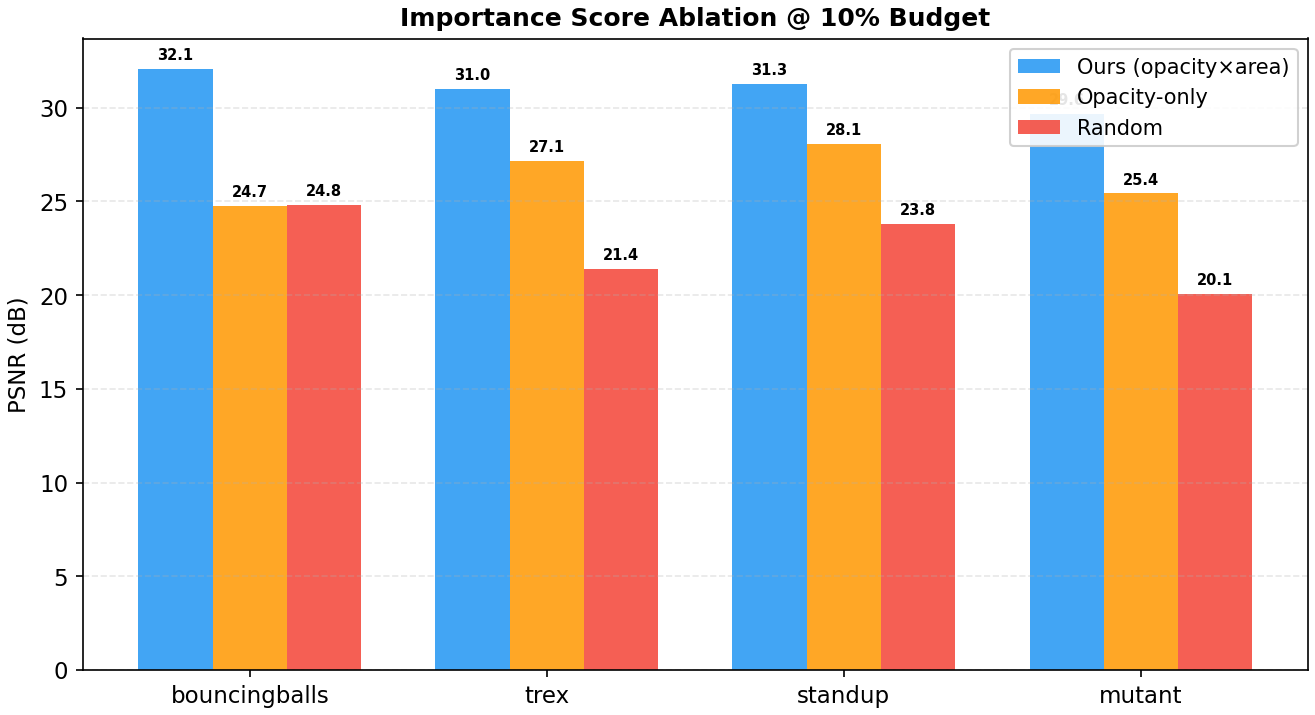
\includegraphics[width=0.82\textwidth]{fig7_ablation_importance.png}
\caption{10\%预算下的重要度评分消融。本文的变形感知评分（不透明度$\times$面积）在四个测试场景上均取得高于纯不透明度排序和随机排序的PSNR。}
\label{fig:importance_ablation}
\end{figure}

图~\ref{fig:importance_ablation}显示，在10\%预算下，本文评分在 bouncingballs、trex、standup 和 mutant 四个场景中分别达到32.1、31.0、31.3和29.6 dB。相比纯不透明度排序，提升幅度分别为7.4、3.9、3.2和4.2 dB；相比随机排序，提升幅度分别为7.3、9.6、7.5和9.5 dB。

这一结果说明，动态4DGS中的基元贡献由可见性和空间覆盖共同决定。不透明度能够反映当前时刻的可见程度，尺度面积则反映基元在图像空间中的影响范围。二者结合后，排序结果更适合低预算前缀截取，也更能保持动态场景中的渲染质量。

\subsubsection{损失函数设计}

本文采用纯前缀损失，使预算分支的图像重建监督集中在排序后的前缀基元上。为了分析完整集损失权重的影响，我们在 bouncingballs 场景上比较了三种设置：Prefix-only（$f_w=0$）、Equal（$f_w=1$）和 Strong（$f_w=2$）。

\begin{figure}[!htbp]
\centering
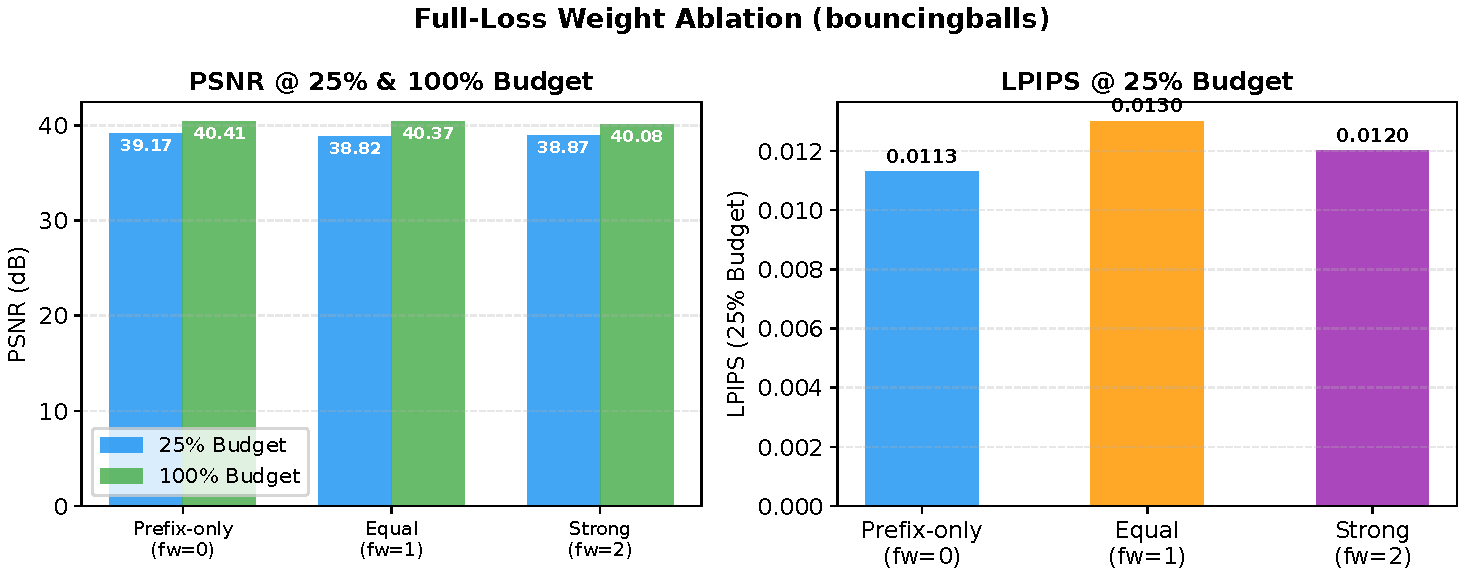
\includegraphics[width=0.82\textwidth]{fig6_ablation_full_loss.pdf}
\caption{bouncingballs场景上的完整集损失权重消融。Prefix-only表示仅使用前缀渲染损失（$f_w=0$），Equal和Strong分别表示加入不同权重的完整集损失。}
\label{fig:loss_ablation}
\end{figure}

图~\ref{fig:loss_ablation}显示，Prefix-only在25\%预算下取得39.17 dB，高于Equal的38.82 dB和Strong的38.87 dB；在100\%预算下，Prefix-only达到40.41 dB，也高于Equal的40.37 dB和Strong的40.08 dB。LPIPS方面，Prefix-only在25\%预算下达到0.0113，优于Equal的0.0130和Strong的0.0120。

这些结果表明，预算分支中的前缀监督对低预算渲染质量具有直接作用。纯前缀损失使优化目标集中在可截取的前缀基元上，从而增强前缀子集的独立渲染能力。与此同时，完整集渲染仍然用于致密化统计，使训练过程保留原始4DGS的基元更新机制。

\subsubsection{静态排序与时间自适应排序}

本文在三个代表性场景上比较了静态排序和时间自适应排序。静态排序在参考时间 $t=0$ 计算一次基元重要度，并在后续帧中复用该排序；时间自适应排序则在每一帧重新计算完整基元集合的重要度。

\begin{table}[!htbp]
\caption{静态排序（参考时间$t=0$）与时间自适应排序在25\%预算下的对比。完全一致的PSNR和完美的秩相关性证实了重要度排序的时间不变性。}
\label{tab:static_ordering}
\centering
\small
\setlength{\tabcolsep}{5pt}
\begin{tabular}{lccc}
\toprule
场景 & 时间自适应 & 静态排序 ($t=0$) & Kendall~$\tau$ \\
\midrule
bouncingballs & 38.82 & 38.82 & 1.0000 \\
standup       & 36.09 & 36.09 & 1.0000 \\
jumpingjacks  & 33.67 & 33.67 & 1.0000 \\
\bottomrule
\end{tabular}
\end{table}

实验结果显示，在所测试的三个场景中，两种排序策略产生了完全一致的前缀选择。25\%预算下，两种策略的PSNR完全相同，Kendall $\tau$ 秩相关系数均为1.0000，top-25\%基元重叠率达到100\%。这一结果表明，在本文测试的场景和预算设置下，基元重要度排序并未随时间发生可观测变化。

因此，推理阶段可以采用一次性静态排序，避免逐帧对完整基元集合重新计算重要度。渲染时，变形网络仍然对被选中的前缀基元运行，以获得当前帧的变形后属性。该策略降低了可变预算推理中的额外排序开销，也简化了部署流程。

\subsection{效率与训练开销}
\label{sec:efficiency}

\subsubsection{渲染速度}

表~\ref{tab:fps}报告了RTX 4080 SUPER上七个D-NeRF合成场景在不同预算比例下的端到端渲染帧率。将预算从100\%降至25\%后，七个场景的平均FPS从78.0提升至114.4，提升幅度为47\%。部分场景在25\%预算下达到更高帧率，例如 jumpingjacks 达到187.8 FPS。

\begin{table}[!htbp]
\caption{不同预算比例下的端到端渲染速度（FPS）。在单张RTX 4080 SUPER上以$800\times800$分辨率测量。}
\label{tab:fps}
\centering
\small
\setlength{\tabcolsep}{5pt}
\begin{tabular}{lccccc}
\toprule
场景 & 10\% & 25\% & 50\% & 75\% & 100\% \\
\midrule
bouncingballs & 70.5 & 71.0 & 67.1 & 56.2 & 50.8 \\
standup       & 77.9 & 68.9 & 69.0 & 70.0 & 59.5 \\
mutant        & 61.4 & 68.5 & 66.6 & 50.2 & 45.1 \\
trex          & 128.1 & 131.0 & 107.7 & 86.7 & 53.3 \\
jumpingjacks  & 159.4 & 187.8 & 153.4 & 150.3 & 137.7 \\
hook          & 110.1 & 135.6 & 106.4 & 108.1 & 83.2 \\
hellwarrior   & 128.7 & 138.1 & 128.3 & 120.2 & 116.7 \\
\midrule
平均          & 105.2 & 114.4 & 99.8 & 91.7 & 78.0 \\
\bottomrule
\end{tabular}
\end{table}

该结果表明，预算截取能够有效降低渲染阶段的基元处理数量，并带来实际速度提升。由于渲染流程中仍包含变形网络前向、光栅化准备和kernel启动等固定开销，FPS并不严格随预算比例线性变化。尽管如此，25\%预算已经能够在多个场景中提供更高吞吐率，并保持较好的渲染质量。

\subsubsection{训练开销}

\begin{figure}[!htbp]
\centering
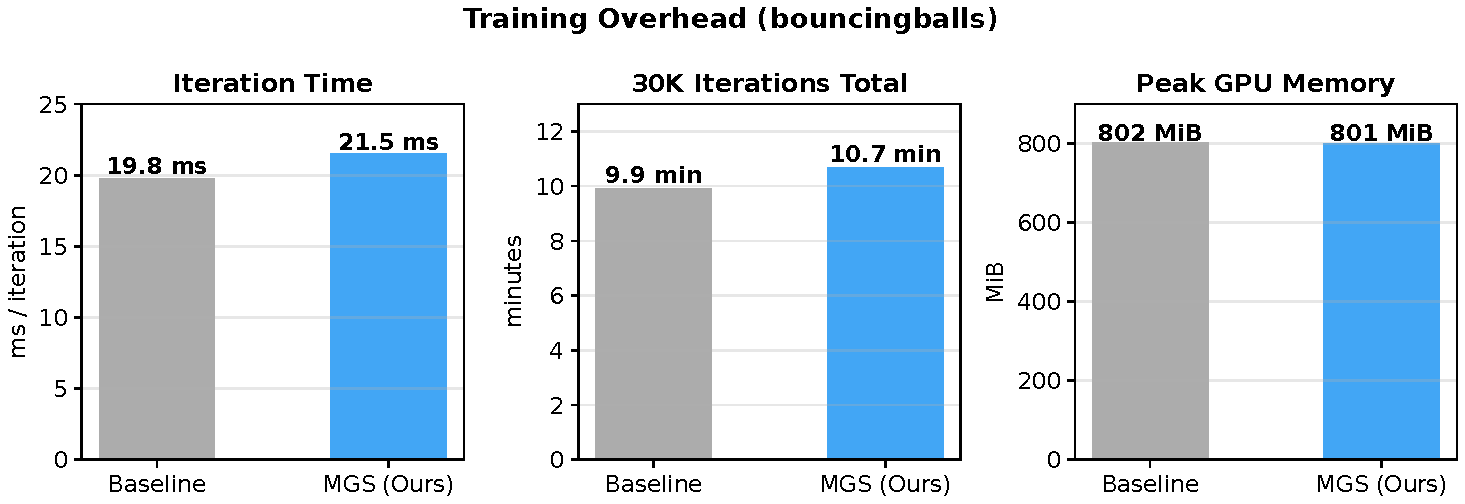
\includegraphics[width=0.82\textwidth]{fig8_training_overhead.pdf}
\caption{bouncingballs场景上的训练开销对比。与标准4DGS训练相比，本文方法的单次迭代时间从19.8 ms增加到21.5 ms，30K次迭代总训练时间从9.9分钟增加到10.7分钟，峰值GPU显存基本保持一致。}
\label{fig:training_overhead}
\end{figure}

图~\ref{fig:training_overhead}展示了随机预算训练带来的额外开销。本文方法的单次迭代时间增加1.7 ms，30K次迭代总训练时间增加0.8分钟。峰值GPU显存从802 MiB变为801 MiB，基本保持一致。

这些结果说明，随机预算训练以较小训练时间增量换取了多预算推理能力。预算分支需要执行重要度计算、top-K选择、前缀渲染以及用于致密化统计的完整集渲染，但这些操作不引入额外可学习参数，也未带来显存增长。结合前述质量和速度结果，本文方法为4DGS模型提供了一种轻量的可变预算训练机制。

% ============================================================================
\section{讨论}
\label{sec:discussion}

\subsection{随机预算训练的作用}

实验结果表明，随机预算训练的主要收益集中在低预算区域。与训练后裁剪相比，本文方法在25\%预算下取得了一致的质量提升，并在10\%至50\%预算区间内表现出更稳定的预算-质量曲线。这说明，可变预算渲染的关键并不只是``如何排序并截取基元''，还在于模型是否在训练阶段真正接触过低预算条件下的前缀子集。

训练后裁剪使用的是已经优化完成的完整模型。该模型在训练过程中始终依赖完整高斯集合完成渲染，因此不同基元之间形成了隐式的协同关系。当推理阶段直接移除一部分基元时，剩余基元并不一定具备独立完成渲染的能力。本文的随机预算训练则在优化过程中反复采样不同规模的前缀子集，使排序靠前的基元持续承担低预算渲染任务。由此得到的前缀基元不仅在完整模型中有用，也能在低预算设置下保持更稳定的表达能力。

这一结果也说明，面向可变预算推理的训练目标与传统压缩目标并不完全相同。传统压缩通常追求某一个固定资源点下的最优模型，而随机预算训练更关注同一模型在多个预算点之间的连续可用性。对于动态场景渲染，这种能力尤其重要，因为实际部署中的计算资源往往会随设备类型、分辨率和交互帧率要求而变化。

\subsection{动态场景中的重要度排序}

重要度评分消融显示，变形后的不透明度与面积代理共同决定了低预算前缀的质量。相比仅使用不透明度排序，本文评分在多个动态场景中取得明显提升。这一结果表明，动态4DGS中的基元贡献不能只从规范空间属性中判断，而需要结合变形后的逐时刻属性。

不透明度反映基元在当前时刻的可见性，面积代理则反映其在图像空间中的影响范围。对于动态场景而言，这两类信息具有互补性。一个基元即使具有较高不透明度，如果尺度很小，可能只影响局部像素；而一个不透明度中等但覆盖范围较大的基元，可能对较大区域的颜色累积产生重要贡献。因此，将二者结合可以更好地选择低预算条件下应当保留的前缀基元。

press场景中的结果进一步揭示了重要度排序的另一个方向。在该真实镜面反射场景中，朴素MGS-4D取得了更高的预算平均PSNR，说明视角相关外观可能会改变基元贡献的判定方式。镜面高光和强视角相关区域并不一定由几何覆盖范围最大的基元主导，部分外观关键基元可能更依赖颜色变化、球谐系数或视角方向上的残差信息。这个现象说明，当前的变形感知评分已经能够覆盖动态几何和可见性因素，但外观感知的重要度估计仍有进一步提升空间。

一个自然的扩展方向是将外观信息纳入评分函数。例如，可以考虑球谐系数能量、颜色方差、视角相关残差或训练过程中的像素贡献统计，使排序同时反映几何覆盖、可见性和外观敏感性。这样的评分可能更适合真实镜面反射场景和高频外观区域，也可以进一步提高可变预算渲染在真实采集数据上的表现。

\subsection{纯前缀损失与动态变形优化}

损失函数消融表明，纯前缀损失在本文测试的动态场景中取得了更稳定的结果。与同时优化前缀损失和完整集损失相比，纯前缀损失使预算分支的优化目标更加集中，直接强化排序靠前基元在低预算条件下的独立渲染能力。

这一现象与动态4DGS的变形场优化有关。前缀子集需要在基元数量受限的情况下完成渲染，因此它鼓励模型将表达能力更多集中到高重要度基元上。完整集损失则关注全部基元共同参与时的重建质量，优化信号更加分散。对于动态场景中的变形场而言，这两类监督可能对基元位置、尺度、不透明度和运动补偿产生不同的优化压力。纯前缀损失减少了这种目标混合，使预算分支更明确地服务于可截取前缀的训练。

需要强调的是，本文并没有移除完整集渲染在训练流程中的作用。在预算约束分支中，完整集渲染仍然用于收集投影半径和可见性过滤等致密化统计信息。也就是说，本文将``图像重建监督''和``致密化统计维护''分开处理：前缀渲染负责预算约束下的图像损失，完整集渲染负责保持原始4DGS致密化过程的稳定性。这一分离使模型能够同时获得低预算监督和稳定的基元更新过程。

\subsection{静态排序的推理优势}

静态排序实验显示，在本文测试的场景和预算设置下，基元重要度排序并未随时间发生可观测变化。静态排序与逐帧时间自适应排序产生了完全一致的前缀选择，Kendall $\tau$ 为1.0000，top-25\%基元重叠率达到100\%。这一结果使推理阶段可以采用一次性排序，而不需要逐帧对完整基元集合重新计算重要度。

这一观察对可变预算部署具有直接意义。推理时，模型只需在参考时间计算一次排序，之后根据目标预算截取对应比例的前缀基元。渲染阶段仍然会对被选中的基元运行变形网络，以获得当前帧的变形后属性；但完整集合上的逐帧重要度评估可以被省去。这样，可变预算推理的额外开销更低，流程也更容易集成到实际渲染系统中。

从实验结果看，排序稳定性可能来自两方面原因。第一，本文的评分使用的是变形后不透明度和尺度面积，而这些属性在训练后对基元整体重要性的排序具有较强一致性。第二，动态场景中的许多核心结构在时间上持续存在，负责主要几何和外观贡献的基元通常不会在短时间内完全改变。因此，即便基元属性随时间发生变化，其相对重要性仍可能保持稳定。

\subsection{复杂运动与预算调度}

在完整预算结果中，部分具有复杂关节运动的场景，如 trex 和 jumpingjacks，出现了相对更明显的PSNR下降。这一现象说明，随机预算扰动会改变动态变形场的优化过程。对于大幅非刚性运动或细粒度关节变化，模型需要同时学习准确运动、局部细节和多预算前缀表达，训练目标之间的平衡更为敏感。

这一结果为后续训练策略提供了改进方向。当前方法在整个训练过程中使用固定的预算分支概率和均匀预算采样。未来可以采用更自适应的预算调度，例如在训练早期使用较高预算帮助模型建立完整结构，在中后期逐步增加低预算采样比例；或者根据场景运动复杂度动态调整预算采样分布，使快速运动和细节区域获得更稳定的优化过程。这样的调度策略有望进一步减小完整预算质量下降，同时保留低预算渲染优势。

\subsection{与压缩和传输方法的互补性}

本文方法关注的是训练阶段的预算适应性，而不是单一压缩率下的模型压缩。因此，它可以与现有高斯压缩、量化和渐进传输方法结合使用。随机预算训练得到的是一个按重要度排序的前缀友好模型；在此基础上，可以继续对高斯属性进行量化、熵编码或分层传输，以进一步降低存储和带宽开销。

这种组合具有实际价值。对于多设备部署，可以先通过随机预算训练获得支持不同基元比例的模型，再根据具体设备选择合适的预算点和压缩强度。对于渐进式传输，排序后的高斯序列也提供了天然的优先级：前缀基元可以优先传输，用于快速获得可用渲染结果；后续基元逐步传输，用于提升细节和完整质量。因此，本文的重要度排序不仅服务于渲染加速，也可能为动态高斯场景的分层存储和渐进加载提供结构信息。

\subsection{计算开销}

本文训练阶段的额外开销主要来自预算分支中的重要度计算、top-K选择、前缀渲染，以及用于致密化统计的完整集渲染。实验显示，在 bouncingballs 场景中，单次迭代时间从19.8 ms增加到21.5 ms，30K次迭代总训练时间从9.9分钟增加到10.7分钟，而峰值GPU显存基本保持不变。

这一结果说明，随机预算训练以较小训练时间增量换取了多预算推理能力。由于该方法不增加模型参数，推理阶段的模型存储结构保持不变；给定目标预算后，只需截取排序后的前缀基元并执行常规4DGS渲染。这种轻量化的设计思路与高效高斯渲染的总体趋势相一致，逐基元优化~\cite{zhang2026dho3dgs}和自适应采样策略~\cite{xu2024efficient}已被证明对实时部署具有实际效果。结合25\%预算下的渲染速度提升，本文方法在训练成本和部署灵活性之间取得了较好的平衡。

% ============================================================================
\section{结论}
\label{sec:conclusion}

本文围绕4D高斯泼溅模型在异构设备部署中的可变预算渲染问题，提出了一种随机预算训练方法。该方法使单一4DGS模型在训练阶段接触不同规模的高斯前缀子集，并在推理阶段根据目标预算直接截取排序后的基元，从而在不重新训练多个模型的情况下实现质量与效率之间的灵活切换。

与直接将静态MGS迁移到动态4DGS不同，本文针对动态场景中的时变属性重新设计了基元选择机制。我们采用变形感知的重要度评分，将HexPlane变形后的不透明度与屏幕空间面积代理结合起来，用于估计基元在当前时刻的渲染贡献。实验表明，该评分相比纯不透明度排序在低预算条件下取得了明显提升，说明动态4DGS中的基元重要度需要结合变形后的逐时刻属性进行估计。

本文还重新考察了随机预算训练中的损失设计。通过将前缀渲染损失与完整集致密化统计分开处理，模型能够在保持原始4DGS致密化流程稳定的同时，直接强化前缀基元在低预算条件下的表达能力。消融结果显示，纯前缀损失在低预算质量、完整预算质量和感知指标上均表现稳定。与此同时，静态排序实验表明，在本文测试的场景和预算设置下，基元重要度排序具有很强的时间稳定性，使推理阶段可以采用一次性排序来降低额外开销。

在9个动态场景上的实验结果表明，本文方法在25\%预算下相较训练后裁剪取得平均+2.0 dB的PSNR提升；当预算从100\%降至25\%时，平均渲染帧率由78.0 FPS提升至114.4 FPS；训练开销仅从19.8 ms/iter增加到21.5 ms/iter，峰值显存基本保持不变。这些结果说明，随机预算训练能够以较小训练成本换取多预算推理能力，为4DGS模型在不同计算平台上的灵活部署提供了一种轻量而实用的机制。

未来工作可以从两个方向继续扩展。一方面，可以将外观信息纳入重要度评分，例如球谐能量、颜色方差或视角相关残差，以进一步提升真实镜面反射场景中的排序质量。另一方面，可以结合自适应预算采样、后训练量化和渐进传输等技术，使预算自适应4DGS在更复杂运动、更长动态序列和带宽受限场景中获得更稳定的表现。

% ============================================================================
\bmhead{声明}

\textbf{资助。} 本研究受到国家自然科学基金（No.~61503005）、教育部人文社会科学基金（No.~22YJAZH002）和北京市自然科学基金（No.~L253018）的资助。

\textbf{利益冲突。} 作者声明不存在利益冲突。

\textbf{数据可用性。} 本研究中使用的D-NeRF和NeRF-DS数据集为公开数据。源代码和训练模型检查点将在论文发表后公开。

\textbf{作者贡献。} 潘宇龙参与了算法实现与数据分析，设计了方法、完成了实验并撰写初稿。张光子提供了技术指导和实验方向。蔡兴泉指导了项目方向并修订了论文。所有作者均已阅读并同意最终稿。

\textbf{伦理批准。} 不适用。

% ============================================================================
\bmhead{作者简介}

% TODO: 在此处插入作者照片（护照风格黑白照片，约4cm宽）。
% 示例：\includegraphics[width=3.5cm]{photo_zhang.pdf}

\textbf{张光子} 
于中国传媒大学获得博士学位，现为北方工业大学人工智能与计算机学院讲师。研究方向包括人工智能、动态场景重建等。

% TODO: 在此处插入作者照片。
% \includegraphics[width=3.5cm]{photo_pan.pdf}

\textbf{潘宇龙} 
于北方工业大学获得学士学位，现为北方工业大学人工智能与计算机学院硕士研究生。研究方向包括三维高斯泼溅、新视角合成和高效深度学习。

% TODO: 在此处插入作者照片。
% \includegraphics[width=3.5cm]{photo_cai.pdf}

\textbf{蔡兴泉} 
于北京航空航天大学获得计算机科学博士学位，现为北方工业大学人工智能与计算机学院教授。研究方向包括计算机图形学、虚拟现实和人机交互。

% ============================================================================
\bibliographystyle{sn-mathphys}
\bibliography{references}

\end{document}
